\documentclass{article}
\usepackage{graphicx,ae}
\usepackage[T1]{fontenc}
\usepackage[latin1]{inputenc}
%\def\rmdefault{mbv}
\usepackage{url}
%\textwidth3in
\let\SetRowColor\relax
%\usepackage[times,symbolmenu,spaced=false,zebra,paperwidth=6in,paperheight=4in]{screenpdf}
\usepackage[]{hyperref}
\title{Simulation of  Energy Loss  Straggling}
\author{Maria Physicist}
\newcommand{\Emax}{\ensuremath{E_{\mathrm{max}}}}
\newcommand{\GEANT}{\texttt{GEANT}}
\begin{document}
\maketitle

\section{Introduction}

Due to the statistical nature of ionisation energy loss, large
fluctuations can occur in the amount of energy deposited by a particle
traversing an absorber element.  Continuous processes such as multiple
scattering and energy loss play a relevant role in the longitudinal
and lateral development of electromagnetic and hadronic
showers, and in the case of sampling calorimeters the
measured resolution can be significantly affected by such fluctuations
in their active layers.  The description of ionisation fluctuations is
characterised by the significance parameter $\kappa$, which is
proportional to the ratio of mean energy loss to the maximum allowed
energy transfer in a single collision with an atomic electron
\[
\kappa =\frac{\xi}{\Emax}
\]
\Emax{}
is the maximum transferable energy in a single collision with
an atomic electron.
\[
\Emax =\frac{2 m_e \beta^2\gamma^2 }
{1 +  2\gamma m_e/m_x + \left ( m_e/m_x\right)^2},
\]
where $\gamma = E/m_x$, $E$ is energy and
$m_x$ the mass of the incident particle, 
$\beta^2 = 1 - 1/\gamma^2$ and $m_e$ is the electron mass. 
$\xi$ comes from the Rutherford scattering cross  section
and is defined as:
\begin{eqnarray*} \xi  = \frac{2\pi z^2 e^4 N_{Av} Z \rho \delta x}
        {m_e \beta^2 c^2 A} =  153.4 \frac{z^2} {\beta^2} \frac{Z}{A}
  \rho \delta x \quad\mathrm{keV},
\end{eqnarray*}
where

\begin{tabular}{ll}
\SetRowColor $z$          & charge of the incident particle \\
\SetRowColor $N_{Av}$     & Avogadro's number \\
\SetRowColor $Z$          & atomic number of the material \\
\SetRowColor $A$          & atomic weight of the material \\
\SetRowColor $\rho$       & density \\
\SetRowColor $ \delta x$  & thickness of the material \\
\end{tabular}

$\kappa$ measures the contribution of the collisions with energy
transfer close to \Emax.  For a given absorber, $\kappa$ tends
towards large values if $\delta x$ is large and/or if $\beta$ is
small.  Likewise, $\kappa$ tends towards zero if $\delta x $ is small
and/or if $\beta$ approaches 1.

The value of $\kappa$ distinguishes two regimes which occur in the
description of ionisation fluctuations :
 
\begin{enumerate}
\item A large number of collisions involving the loss of all or most
  of the incident particle energy during the traversal of an absorber.
  
  As the total energy transfer is composed of a multitude of small
  energy losses, we can apply the central limit theorem and describe
  the fluctuations by a Gaussian distribution.  This case is
  applicable to non-relativistic particles and is described by the
  inequality $\kappa > 10 $ (i.e. when the mean energy loss in the
  absorber is greater than the maximum energy transfer in a single
  collision).
  
\item Particles traversing thin counters and incident electrons under
  any conditions.
  
  The relevant inequalities and distributions are $ 0.01 < \kappa < 10
  $, Vavilov distribution, and $\kappa < 0.01 $, Landau distribution.
\end{enumerate}

An additional regime is defined by the contribution of the collisions
with low energy transfer which can be estimated with the relation
$\xi/I_0$, where $I_0$ is the mean ionisation potential of the atom.
Landau theory assumes that the number of these collisions is high, and
consequently, it has a restriction $\xi/I_0 \gg 1$.  In \GEANT{}
(see URL \url{http://wwwinfo.cern.ch/asdoc/geant/geantall.html}), the
limit of Landau theory has been set at $\xi/I_0 = 50$.  Below this
limit special models taking into account the atomic structure of the
material are used.  This is important in thin layers and gaseous
materials.  \autoref{fg:phys332-1} shows the behaviour of $\xi/I_0$
as a function of the layer thickness for an electron of 100 keV and 1
GeV of kinetic energy in Argon, Silicon and Uranium.

\begin{figure}
   \centering
   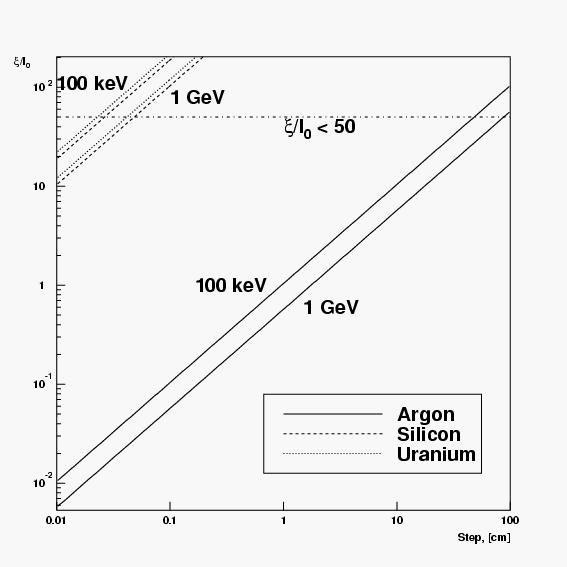
\includegraphics[width=.6\linewidth]{phys1}
   \caption{The variable $\xi/I_0$ can be used to measure the 
            validity range of the Landau theory. It depends
            on the type and energy of the particle, $Z$, $A$
            and the ionisation potential of the material and
            the layer thickness. 
            }
    \label{fg:phys332-1}
\end{figure}

In the following sections, the different theories and models for the
energy loss fluctuation are described. First, the Landau theory and
its limitations are discussed, and then, the Vavilov and Gaussian
straggling functions and the methods in the thin layers and gaseous
materials are presented.

\section{Landau theory}
\label{sec:phys332-1}

For a particle of mass $m_x$ traversing a thickness of material
$\delta x $, the Landau probability distribution may be written in
terms of the universal Landau function $\phi(\lambda)$
as\cite{bib-LAND}:
\begin{eqnarray*}
f( \epsilon , \delta x ) & = &\frac{1}{\xi} \phi ( \lambda )    
\end{eqnarray*}
where
\begin{eqnarray*}
\phi(\lambda )& = & \frac{1} {2 \pi i}\int^{c+i\infty}_{c-i\infty}
\exp \left ( u \ln u + \lambda u \right ) du \hspace{2cm} c \geq 0 \\
\lambda       & = & \frac{\epsilon  -\bar{\epsilon} }{\xi}
  - \gamma' - \beta^2 - \ln \frac{\xi}{\Emax}          \\
\gamma' & = & 0.422784\dots = 1 - \gamma \\
\gamma             & = & 0.577215\dots \mbox{(Euler's constant)}   \\
\bar{\epsilon}  & = & \mbox{average energy loss}                    \\
\epsilon      & = & \mbox{actual energy loss}
\end{eqnarray*}

\subsection{Restrictions}

The Landau formalism makes two restrictive assumptions :
\begin{enumerate}
\item The typical energy loss is small compared to the maximum energy
  loss in a single collision.  This restriction is removed in the
  Vavilov theory (see \autoref{vavref}).
\item The typical energy loss in the absorber should be large compared
  to the binding energy of the most tightly bound electron.  For
  gaseous detectors, typical energy losses are a few keV which is
  comparable to the binding energies of the inner electrons.  In such
  cases a more sophisticated approach which accounts for atomic energy
  levels\cite{bib-TALM} is necessary to accurately simulate data
  distributions. In \GEANT, a parameterised model by L.  Urb\'{a}n is
  used (see section \ref{urban}).
\end{enumerate}

In addition, the average value of the Landau distribution is infinite.
Summing the Landau fluctuation obtained to the average energy from the
$dE/dx$ tables, we obtain a value which is larger than the one coming
from the table.  The probability to sample a large value is small, so
it takes a large number of steps (extractions) for the average
fluctuation to be significantly larger than zero. This introduces a
dependence of the energy loss on the step size which can affect
calculations.

A solution to this has been to introduce a limit on the value of the
variable sampled by the Landau distribution in order to keep the
average fluctuation to 0. The value obtained from the \texttt{GLANDO}
routine is:
\[
\delta dE/dx = \epsilon - \bar{\epsilon} = \xi ( \lambda - \gamma'
+\beta^2 +\ln \frac{\xi}{\Emax})
\]
In order for this to have average 0, we must impose that:
\[
\bar{\lambda} = -\gamma' - \beta^2 -\ln \frac{\xi}{\Emax}
\]

This is realised introducing a $\lambda_{\mathrm{max}}(\bar{\lambda})$
such that if only values of $\lambda \leq \lambda_{\mathrm{max}}$ are
accepted, the average value of the distribution is $\bar{\lambda}$.

A parametric fit to the universal Landau distribution has been
performed, with following result:
\[
\lambda_{\mathrm{max}} = 0.60715 +
     1.1934\bar{\lambda}+(0.67794+0.052382\bar{\lambda})
     \exp(0.94753+0.74442\bar{\lambda})
\]
only values smaller than $\lambda_{\mathrm{max}}$ are accepted, otherwise the
distribution is resampled.



\section{Vavilov theory}
\label{vavref}

Vavilov\cite{bib-VAVI} derived a more accurate straggling distribution
by introducing the kinematic limit on the maximum transferable energy
in a single collision, rather than using $ \Emax = \infty $.
Now we can write\cite{bib-SCH1}:
\begin{eqnarray*}
f \left ( \epsilon, \delta s \right ) & = & \frac{1}{\xi} \phi_{v}
\left ( \lambda_{v}, \kappa, \beta^{2} \right )
\end{eqnarray*}
where
\begin{eqnarray*}
\phi_{v} \left ( \lambda_{v}, \kappa, \beta^{2} \right ) & = &
\frac{1}{2 \pi i} \int^{c+i\infty}_{c-i\infty}\phi \left( s \right ) 
e^{\lambda s} ds \hspace{2cm} c \geq 0 \\
\phi \left ( s \right ) & = & 
\exp \left [ \kappa ( 1 + \beta^{2}\gamma ) \right ]
~ \exp \left [ \psi \left ( s \right ) \right ], \\
\psi \left ( s \right )  & = & s \ln \kappa + ( s + \beta^{2} \kappa )
\left [ \ln (s/\kappa) + E_{1} (s/\kappa) \right ] - \kappa e^{-s/\kappa}, 
\end{eqnarray*}
and
\begin{eqnarray*}
E_{1}(z) & = & \int^{\infty}_{z} t^{-1} e^{-t} dt 
\mbox{\hspace{1cm} (the exponential integral)} \\
\lambda_v & = & \kappa \left [ \frac{\epsilon - \bar{\epsilon}}{\xi}
- \gamma' - \beta^2 \right]
\end{eqnarray*}

The Vavilov parameters are simply related to the Landau parameter by
$\lambda_L = \lambda_v/\kappa - \ln\kappa $. It can be shown that as
$\kappa \rightarrow 0$, the distribution of the variable $\lambda_L$
approaches that of Landau. For $\kappa \leq 0.01$ the two
distributions are already practically identical. Contrary to what many
textbooks report, the Vavilov distribution \emph{does not} approximate
the Landau distribution for small $\kappa$, but rather the
distribution of $\lambda_L$ defined above tends to the distribution of
the true $\lambda$ from the Landau density function.  Thus the routine
\texttt{GVAVIV} samples the variable $\lambda_L$ rather than
$\lambda_v$.  For $\kappa \geq 10$ the Vavilov distribution tends to a
Gaussian distribution (see next section).
 
\section{Gaussian Theory}
 
Various conflicting forms have been proposed for Gaussian straggling
functions, but most of these appear to have little theoretical or
experimental basis.  However, it has been shown\cite{bib-SELT} that
for $\kappa \geq 10 $ the Vavilov distribution can be replaced by a
Gaussian of the form :
\begin{eqnarray*}
f( \epsilon , \delta s)  \approx \frac{1}
{\xi \sqrt{\frac{2 \pi}{\kappa} \left( 1 - \beta^2/2 \right)}}
   \exp \left [ \frac{( \epsilon - \bar{\epsilon} )^2}{2} \frac{\kappa}
   {\xi^2 (1- \beta^2/2)}\right ]
\end{eqnarray*}
thus implying 
\begin{eqnarray*}
\mathrm{mean} & = & \bar{\epsilon} \\
\sigma^2      & = & \frac{\xi^2}{\kappa} (1-\beta^2/2) = \xi
                    \Emax (1-\beta^2/2)
\end{eqnarray*}

\section{Urb\'an model}
\label{urban}

The method for computing restricted energy losses with $\delta$-ray
production above given threshold energy in \GEANT{} is a Monte
Carlo method that can be used for thin layers.  It is fast and it can
be used for any thickness of a medium.  Approaching the limit of the
validity of Landau's theory, the loss distribution approaches smoothly
the Landau form as shown in \autoref{fg:phys332-2}.
\begin{figure}
   \centering
   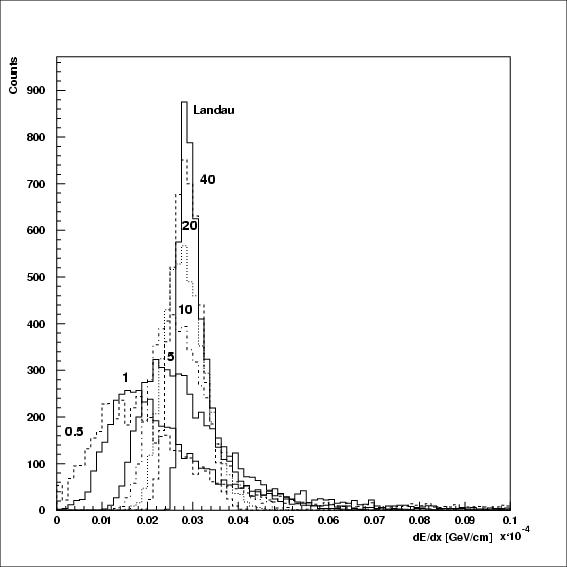
\includegraphics[width=.6\linewidth]{phys2}
   \caption{Energy loss distribution for a 3 GeV electron in
     Argon as given by standard \GEANT.  The width of the layers is
     given in centimeters.}
    \label{fg:phys332-2}
\end{figure}

It is assumed that the atoms have only two energy levels with binding
energy $E_1$ and $E_2$.  The particle--atom interaction will then be
an excitation with energy loss $E_1$ or $E_2$, or an ionisation with
an energy loss distributed according to a function $g(E) \sim 1/E^2$:
\begin{equation}
g(E) = \frac{(\Emax + I)I}{\Emax} \frac{1}{E^2}
\end{equation}

The macroscopic cross-section for excitations ($i=1,2$) is
\begin{equation}
\label{eq:sigex}
\Sigma_i = C \frac{f_i}{E_i} \frac{\ln (2 m \beta^2 \gamma^2/E_i) - \beta^2}
             {\ln (2 m \beta^2 \gamma^2/ I) - \beta^2}(1-r)
\end{equation}
and the macroscopic cross-section for ionisation is
\begin{equation}
\label{eq:sigion}
\Sigma_3 = C \frac{\Emax}{I(\Emax+I) \ln(\frac{\Emax+I}{I})}
           ~ r
\end{equation}
\Emax{} is the \GEANT{} cut for $\delta$-production, or the maximum
energy transfer minus mean ionisation energy, if it is smaller than
this cut-off value.  The following notation is used:

\begin{tabular}{ll}
\SetRowColor $r, C$          & parameters of the model \\
\SetRowColor $E_i$           & atomic energy levels \\
\SetRowColor $I$             & mean ionisation energy \\
\SetRowColor ${f_i}$         & oscillator strengths 
\end{tabular}

The model has the parameters $f_i$, $E_i$, $C$ and $r ~(0\leq r\leq
1)$.  The oscillator strengths $f_i$ and the atomic level energies
$E_i$ should satisfy the constraints
\begin{eqnarray}
f_1 + f_2 & = & 1  \label{eq:fisum}\\
f_1 \ln E_1 + f_2 \ln E_2 & = & \ln I \label{eq:flnsum}
\end{eqnarray}
The parameter $C$ can be defined with the help of the mean energy loss
$dE/dx$ in the following way: The numbers of collisions ($n_i$, i =
1,2 for the excitation and 3 for the ionisation) follow the Poisson
distribution with a mean number $ \langle n_i \rangle $. In a step
$\Delta x$ the mean number of collisions is
\begin{equation}
\langle n_i \rangle = \Sigma_i \Delta x
\end{equation}
The mean energy loss $dE/dx$ in a step is the sum of the excitation
and ionisation contributions
\begin{equation}
\frac{dE}{dx} \Delta x = \left[ \Sigma_1 E_1 + \Sigma_2 E_2 +
                          \Sigma_3 \int_{I}^{\Emax+I} E~g(E)~dE \right]
                         \Delta x
\end{equation}
From this, using the equations (\ref{eq:sigex}), (\ref{eq:sigion}),
(\ref{eq:fisum}) and (\ref{eq:flnsum}), one can define the parameter
$C$
\begin{equation}
C = \frac{dE}{dx}
\end{equation}

The following values have been chosen in \GEANT{} for the other
parameters:
\[ 
\begin{array}{lcl}
f_2 = \left\{ \begin{array}{ll}
             0   & \mathrm{if} Z \leq 2 \\
             2/Z & \mathrm{if} Z > 2 \\
             \end{array} \right.    & \Rightarrow & f_1 = 1 - f_2 \\
E_2 = 10 Z^2 \mathrm{eV}  & \Rightarrow & E_1 = \left(\frac{I}{E_{2}^{f_2}}
                                              \right)^{\frac{1}{f_1}} \\
r  = 0.4 & & \\
\end{array}
\]
With these values the atomic level $E_2$ corresponds approximately
the K-shell energy of the atoms and $Zf_2$ the number of K-shell
electrons. $r$ is the only variable which can be tuned freely. It
determines the relative contribution of ionisation and
excitation to the energy loss.

The energy loss is computed with the assumption that the step length
(or the relative energy loss) is small, and---in consequence---the
cross-section can be considered constant along the path length.  The
energy loss due to the excitation is
\begin{equation}
\Delta E_e = n_1 E_1 + n_2 E_2
\end{equation}
where $n_1$ and $n_2$ are sampled from Poisson distribution as
discussed above.  The loss due to the ionisation can be generated from
the distribution $g(E)$ by the inverse transformation method:
\begin{eqnarray}
u = F(E) &  = & \int_{I}^E g(x) dx \nonumber \\
E = F^{-1}(u) & = & \frac{I}{1 - u \frac {\Emax}{\Emax+I}} \\
\end{eqnarray}
where $u$ is a uniform random number between $F(I)=0$ and
$F(\Emax+I)=1$.  The contribution from the ionisations will be
\begin{equation}
\Delta E_i  = \sum_{j=1}^{n_3} \frac{I}
              {1 - u_j \frac {\Emax}{\Emax + I}}
\end{equation}
where $n_3$ is the number of ionisation (sampled from Poisson
distribution). The energy loss in a step will then be $\Delta E =
\Delta E_e + \Delta E_i$.


\subsection{Fast simulation for $n_3 \geq 16$}

If the number of ionisation $n_3$ is bigger than 16, a faster sampling
method can be used. The possible energy loss interval is divided in
two parts: one in which the number of collisions is large and the
sampling can be done from a Gaussian distribution and the other in
which the energy loss is sampled for each collision.  Let us call the
former interval $[I, \alpha I]$ the interval A, and the latter
$[\alpha I,\Emax]$ the interval B.  $\alpha$ lies between 1 and
$\Emax/I$.  A collision with a loss in the interval A happens with
the probability
\begin{equation}
\label{eq:phys332-5}
P(\alpha) = \int_I^{\alpha I} g(\!E\!) \, dE =
            \frac {( \Emax + I) (\alpha - 1)}{\Emax \alpha}
\end{equation}
The mean energy loss and the standard deviation for this type
of collision are
\begin{equation}
\langle \Delta E(\alpha) \rangle = \frac{1}{P(\alpha)} 
        \int_I^{\alpha I} E \, g(\!E\!) \, dE =
        \frac{I \alpha \ln \alpha}{\alpha - 1}
\end{equation}
and
\begin{equation}
\sigma^2(\alpha) = \frac{1}{P(\alpha)}
        \int_I^{\alpha I} E^2 \, g(\!E\!) \, dE =
        I^2 \alpha \left( 1 - \frac{\alpha \ln \! ^2 \alpha}{(\alpha - 1)^2} \right)
\end{equation}
If the collision number is high , we assume that the number of the
type A collisions can be calculated from a Gaussian distribution
with the following mean value and standard deviation:
\begin{eqnarray}
\label{eq:phys332-1}
\langle n_A \rangle & = & n_3 P(\alpha) \\
\label{eq:phys332-2}
\sigma_A^2     & = & n_3 P(\alpha) ( 1 - P(\alpha))
\end{eqnarray}
It is further assumed that the energy loss in these collisions
has a Gaussian distribution with
\begin{eqnarray}
\label{eq:phys332-3}
\langle \Delta E_A \rangle & = & n_A  \langle \Delta E(\alpha) \rangle \\
\label{eq:phys332-4}
\sigma_{E,A}^2             & = & n_A \sigma^2(\alpha)
\end{eqnarray}
The energy loss of these collision can then be sampled from the
Gaussian distribution.

The collisions where the energy loss is in the interval B are sampled
directly from
\begin{equation}
\Delta E_B = \sum_{i=1}^{n_3 - n_A} \frac{\alpha I}
            {1 - u_i \frac{\Emax + I - \alpha I}{\Emax + I}}
\end{equation}
The total energy loss is the sum of these two types of collisions:
\begin{equation}
\Delta E =  \Delta E_A + \Delta E_B
\end{equation}

The approximation of equations (\ref{eq:phys332-1}),
(\ref{eq:phys332-2}), (\ref{eq:phys332-3}) and (\ref{eq:phys332-4})
can be used under the following conditions:
\begin{eqnarray}
\label{eq:phys332-6}
\langle n_A \rangle - c \, \sigma_A            & \geq & 0 \\
\label{eq:phys332-7}
\langle n_A \rangle + c \, \sigma_A            & \leq & n_3 \\
\label{eq:phys332-8}
\langle \Delta E_A \rangle - c \, \sigma_{E,A} & \geq & 0
\end{eqnarray}
where $c \geq 4$. From the equations (\ref{eq:phys332-5}),
(\ref{eq:phys332-1}) and (\ref{eq:phys332-3}) and from the conditions
(\ref{eq:phys332-6}) and (\ref{eq:phys332-7}) the following limits can
be derived:
\begin{equation}
\alpha_{\mathrm{min}} = \frac{(n_3 + c^2)(\Emax+I)}
                      {n_3 (\Emax + I) + c^2 I} \; \leq \alpha \; \leq
\alpha_{\mathrm{max}} = \frac{(n_3 + c^2)(\Emax+I)}
                      {c^2 (\Emax + I) + n_3 I}
\end{equation}
This conditions gives a lower limit to number of the ionisations $n_3$
for which the fast sampling can be done:
\begin{equation}
n_3 \; \geq \; c^2
\end{equation}
As in the conditions (\ref{eq:phys332-6}), (\ref{eq:phys332-7}) and
(\ref{eq:phys332-8}) the value of $c$ is as minimum 4, one gets $n_3
\; \geq 16$. In order to speed the simulation, the maximum value is
used for $\alpha$.

The number of collisions with energy loss in the interval B (the
number of interactions which has to be simulated directly) increases
slowly with the total number of collisions $n_3$. The maximum number
of these collisions can be estimated as
\begin{equation}
n_{B,max} = n_3 - n_{A,min} \approx n_3 (\langle n_A \rangle 
            - \sigma_A)
\end{equation}
From the previous expressions for $\langle n_A \rangle$ and $\sigma_A$
one can derive the condition
\begin{equation}
n_B \; \leq \; n_{B,max} = \frac{2 n_3 c^2}{n_3+c^2}
\end{equation}
The following values are obtained with $c=4$:

\begin{tabular}{llcrr}
$n_3$  & $n_{B,max}$ & & $n_3$  & $n_{B,max}$\\ 
\hline
\SetRowColor 16   & 16      & & 200  & 29.63\\
\SetRowColor 20   & 17.78   & & 500  & 31.01 \\
\SetRowColor 50   & 24.24   & & 1000 & 31.50 \\
\SetRowColor 100  & 27.59   & & $\infty$ & 32.00
\end{tabular}

\subsection{Special sampling for lower part of the spectrum}

If the step length is very small ($\leq 5$ mm in gases, $\leq$ 2-3
$\mu$m in solids) the model gives 0 energy loss for some events.  To
avoid this, the probability of 0 energy loss is computed
\begin{equation}
P( \Delta E=0) = e^{-( \langle n_1 \rangle + \langle n_2 \rangle
                     + \langle n_3 \rangle )}
\end{equation}
If the probability is bigger than 0.01 a special sampling is done,
taking into account the fact that in these cases the projectile
interacts only with the outer electrons of the atom.  An energy level
$E_0 = 10$ eV is chosen to correspond to the outer electrons. The mean
number of collisions can be calculated from
\begin{equation}
\langle n \rangle = \frac{1}{E_0} \frac{dE}{dx} \Delta x
\end{equation}
The number of collisions $n$ is sampled from Poisson distribution.
In the case of the thin layers, all the collisions are considered as
ionisations and the energy loss is computed as
\begin{equation}
\Delta E = \sum_{i=1}^n \frac{E_0}
          {1 - \frac {\Emax}{\Emax + E_0} u_i}
\end{equation}


\begin{thebibliography}{10}
\bibitem{bib-LAND}
L.Landau.
\newblock On the Energy Loss of Fast Particles by Ionisation.
\newblock Originally published in \emph{J. Phys.}, 8:201, 1944.
\newblock Rerpinted in D.ter Haar, Editor, \emph{L.D.Landau, Collected
  papers}, page 417.  Pergamon Press, Oxford, 1965.

\bibitem{bib-SCH1}
B.Schorr.
\newblock Programs for the Landau and the Vavilov distributions and the
  corresponding random numbers.
\newblock \emph{Comp. Phys. Comm.}, 7:216, 1974.

\bibitem{bib-SELT}
S.M.Seltzer and M.J.Berger.
\newblock Energy loss straggling of protons and mesons. 
\newblock In \emph{Studies in Penetration of Charged Particles in
  Matter}, Nuclear Science Series~39, Nat. Academy of Sciences,
  Washington DC, 1964.

\bibitem{bib-TALM}
R.Talman.
\newblock On the statistics of particle identification using ionization.
\newblock \emph{Nucl. Inst. Meth.}, 159:189, 1979.

\bibitem{bib-VAVI}
P.V.Vavilov.
\newblock Ionisation losses of high energy heavy particles.
\newblock \emph{Soviet Physics JETP}, 5:749, 1957.

\end{thebibliography}

\end{document}
